\section{CLgen: Benchmark Synthesis}%
% \label{sec:TODO}

This section introduces CLgen, a tool for synthesizing OpenCL benchmarks, and an accompanying host driver for executing synthetic benchmarks for gathering performance data for predictive modeling. While we demonstrate our approach using OpenCL, it is language agnostic. Our tool CLgen learns the semantics and structure from over a million lines of hand-written code from GitHub, and synthesizes programs through a process of iterative model sampling. We use a host driver to execute the synthesized programs to gather performance data for use in predictive modeling. Figure~\ref{fig:clgen-pipeline} provides an overview of the program synthesis and execution pipeline. Our approach extends the state of the art by providing a general-purpose solution for benchmark synthesis, leading to better and more accurate predictive models.

In the course of evaluating our technique against prior work we discovered that it is also useful for evaluating the quality of features. Since we are able to cover the space so much more finely than the prior work, which only used standard benchmark suites, we are able to find multiple programs with identical feature values but different best heuristic values. This indicates that the features are not sufficiently discriminative and should be extended with more information to allow those programs to be separated. We go on to show that doing this significantly increases the performance of the learned heuristics. We expect that our technique will be valuable for feature designers.

\begin{figure}
	\centering%
	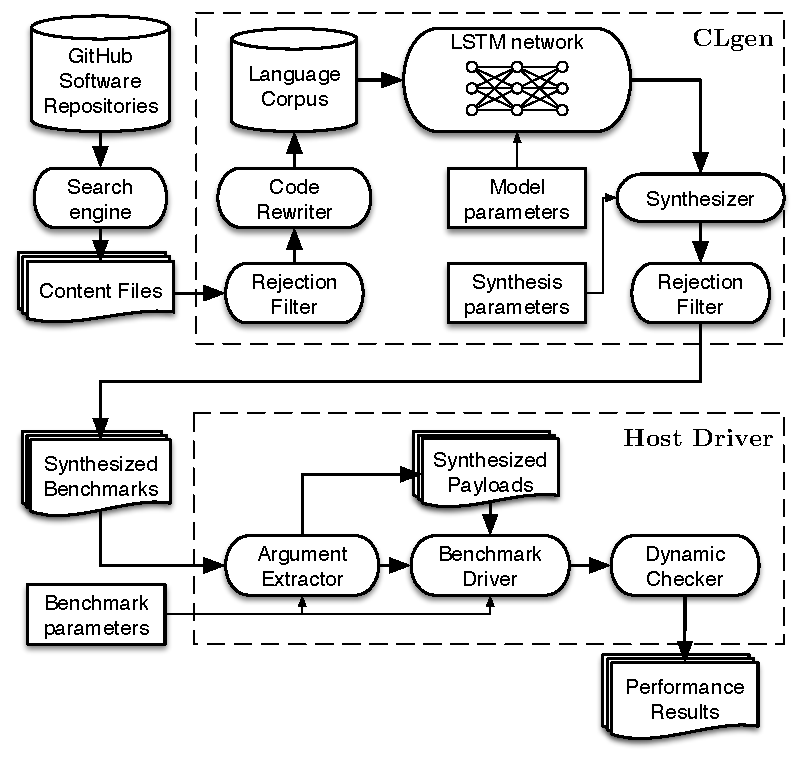
\includegraphics[width=.77\columnwidth]{img/pipeline}%
	\caption{Benchmark synthesis and execution pipeline.}%
	\label{fig:clgen-pipeline}
\end{figure}

\todo[inline]{End of inlined overview section}

CLgen is an undirected, general-purpose program synthesizer for OpenCL. It adopts and augments recent advanced techniques from deep learning to learn over massive codebases. In contrast to existing grammar and template based approaches, CLgen is entirely probabilistic. The system \emph{learns} to program using neural networks which model the semantics and usage of a huge corpus of code fragments in the target programming language. This section describes the assembly of an OpenCL language corpus, the application of deep learning over this corpus, and the process of synthesizing programs.

\subsection{An OpenCL Language Corpus}

Deep learning requires large datasets~\cite{LeCun2015}. For the purpose of modeling a programming language, this means assembling a very large collection of real, hand-written source codes. We assembled OpenCL codes by mining public repositories on the popular code hosting site GitHub.

This is itself a challenging task since OpenCL is an embedded language, meaning device code is often difficult to untangle since GitHub does not presently recognize it as a searchable programming language. We developed a search engine which attempts to identify and download standalone OpenCL files through a process of file scraping and recursive header inlining. The result is a 2.8 million line dataset of 8078 ``content files'' which potentially contain OpenCL code, originating from 793 GitHub repositories.

We prune the raw dataset extracted from GitHub using a custom toolchain we developed for rejection filtering and code rewriting, built on LLVM.

\subsubsection{Rejection Filter}\label{sec:rejection-filter} The rejection filter accepts as input a content file and returns whether or not it contains compilable, executable OpenCL code. To do this we attempt to compile the input to NVIDIA PTX bytecode and perform static analysis to ensure a minimum static instruction count of three. We discard any inputs which do not compile or contain fewer than three instructions.

During initial development it became apparent that isolating the OpenCL device code leads to a higher-than-expected discard rate (that is, seemingly valid OpenCL files being rejected). Through analyzing 148k lines of compilation errors, we discovered a large number of failures caused by undeclared identifiers --- a result of isolating device code --- 50\% of undeclared identifier errors in the GitHub dataset were caused by only 60 unique identifiers. To address this, we developed a \emph{shim header} which contains inferred values for common type definitions (e.g. \texttt{FLOAT\_T}), and common constants (e.g. \texttt{WGSIZE}), shown in Listing~\ref{lst:shim}.

Injecting the shim decreases the discard rate from 40\% to 32\%, responsible for an additional 88k lines of code in the final language corpus. The resulting dataset is 2.0 million lines of compilable OpenCL source code.

\subsubsection{Code Rewriter} Programming languages have few of the issues of semantic interpretation present in natural language, though there remains many sources of variance at the syntactic level. For example, the presence and content of comments in code, and the choice of identifying names given to variables. We consider these  ambiguities to be \emph{non-functional variance}, and developed a tool to normalize code of these variances so as to make the code more amenable to machine learning. This is a three step process: %
%
\begin{enumerate}
  \item The source is pre-processed to remove macros, conditional compilation, and source comments. %
  \item Identifiers are rewritten to have a short but unique name based on their order of appearance, using the sequential series $\{a,\allowbreak b,\allowbreak c,\allowbreak \ldots,\allowbreak aa,\allowbreak ab,\allowbreak ac,\allowbreak \ldots\}$ for variables and $\{A,\allowbreak B,\allowbreak C,\allowbreak \ldots,\allowbreak AA,\allowbreak AB,\allowbreak AC,\allowbreak \ldots\}$ for functions. This process isolates the syntactic structure of the code, and unlike prior work~\cite{Allamanis2013a}, our rewrite method preserves program behavior. Language built-ins (e.g. \texttt{get\_global\_id}, \texttt{asin}) are not rewritten.%
  \item A variant of the Google C++ code style is enforced to ensure consistent use of braces, parentheses, and white space.
\end{enumerate}


\lstset{language=C}
\begin{lstlisting}[%
  label={lst:shim},%
  float,%
  caption={The \emph{shim} header file, providing inferred type aliases and constants for OpenCL on GitHub.}%
]
/* Enable OpenCL features */
#define cl_clang_storage_class_specifiers
#define cl_khr_fp64
#include <clc/clc.h>

/* Inferred types */
typedef float FLOAT_T;
typedef unsigned int INDEX_TYPE;
... (36 more)

/* Inferred constants */
#define M_PI 3.14025
#define WG_SIZE 128
... (185 more)
\end{lstlisting}

\noindent %
An example of the code rewriting process is shown in Listings~\ref{lst:code-rewriting-before} and~\ref{lst:code-rewriting-after}. A side effect of this process is a reduction in code size, largely due to the removal of comments and excess white space. The final language corpus contains 1.3 million lines of transformed OpenCL, consisting of 9487 kernel functions. Identifier rewriting reduces the bag-of-words vocabulary size by 84\%.

\subsection{Learning OpenCL}\label{sec:ml}

Generating valid, executable program code is an ambitious and challenging goal for unsupervised machine learning. We employ state of the art deep language modeling techniques to achieve this task.

\lstset{language=[OpenCL]C}
\begin{lstlisting}[%
label={lst:code-rewriting-before},%
float,%
caption={An example content file downloaded from GitHub prior to code rewriting.}%
]
#define DTYPE float
#define ALPHA(a) 3.5f * a
inline DTYPE ax(DTYPE x) { return ALPHA(x); }

__kernel void saxpy( /* SAXPY kernel */
    __global DTYPE *input1,
    __global DTYPE *input2,
    const int nelem)
{
     unsigned int idx = get_global_id(0);
     // = ax + y
     if (idx < nelem) {
         input2[idx] += ax(input1[idx]); }}
\end{lstlisting}

\lstset{language=[OpenCL]C}
\begin{lstlisting}[%
label={lst:code-rewriting-after},%
float,%
caption={The code listing from~\ref{lst:code-rewriting-before} after code rewriting.}%
]
inline float A(float a) {
  return 3.5f * a;
}

__kernel void B(__global float* b, __global float* c, const int d) {
  unsigned int e = get_global_id(0);

  if (e < d) {
    c[e] += A(b[e]);
  }
}
\end{lstlisting}

The Long Short-Term Memory (LSTM) architecture of Recurrent Neural Network~\cite{Sundermeyer2012,Mikolov2015} is used to learn a character-level language model over the corpus of OpenCL compute kernels. The LSTM network architecture comprises recurrent layers of \emph{memory cells}, each consisting of an input, output, and forget gate, and an output layer providing normalized probability values from a 1-of-K coded vocabulary~\cite{Graves}.

We use a 3-layer LSTM network with 2048 nodes per layer, implemented in Torch. We train this 17-million parameter model using \textit{Stochastic Gradient Descent} for 50 epochs, using an initial learning rate of 0.002, decaying by a factor of one half every 5 epochs. Training took three weeks on a single machine using an NVIDIA GTX Titan, with a final model size of 648MB. Training the network is a one-off cost, and can be parallelized across devices. The trained network can be deployed to lower-compute machines for use.

\subsection{Synthesizing OpenCL}

We synthesize OpenCL compute kernels by iteratively sampling the learned language model. We implemented two modes for model sampling: the first involves providing an \emph{argument specification}, stating the data types and modifiers of all kernel arguments. When an argument specification is provided, the model synthesizes kernels matching this signature. In the second sampling mode this argument specification is omitted, allowing the model to synthesize compute kernels of arbitrary signatures, dictated by the distribution of argument types within the language corpus.

In either mode we generate a \emph{seed} text, and sample the model, character by character, until the end of the compute kernel is reached, or until a predetermined maximum number of characters is reached. Algorithm~\ref{alg:synthesis} illustrates this process. The same rejection filter described in Section~\ref{sec:rejection-filter} then either accepts or rejects the sample as a candidate synthetic benchmark. Listing~\ref{lst:ex} shows three examples of unique compute kernels generated in this manner from an argument specification of three single-precision floating-point arrays and a read-only signed integer. We evaluate the quality of synthesized code in Section~\ref{sec:eval}.

\begin{algorithm}[t]
\begin{algorithmic}[1]
\Require LSTM model $M$, maximum kernel length $n$.
\Ensure Completed sample string $S$.
\State $S \gets$``\texttt{\_\_kernel void A(const int a) \{}''\algorithmiccomment{Seed text}
\State $d \gets 1$\algorithmiccomment{Initial code block depth}
\For{$i \gets |S|$ \textbf{to} $n$}
  \State $c \gets predictcharacter(M, S)$\algorithmiccomment{Generate new character}
  \If{$c = $``\texttt{\{}''}
    \State $d \gets d+1$\algorithmiccomment{Entered code block, increase depth}
  \ElsIf{$c = $``\texttt{\}}''}
    \State $d \gets d-1$\algorithmiccomment{Exited code block, decrease depth}
  \EndIf
  \State $S \gets S + c$\algorithmiccomment{Append new character}
  \If{$depth = 0$}
    \State \textbf{break}\algorithmiccomment{Exited function block, stop sampling}
  \EndIf

\EndFor
\end{algorithmic}
\caption{Sampling a candidate kernel from a seed text.}
\label{alg:synthesis}
\end{algorithm}

\lstset{language=[OpenCL]C}
\begin{figure}
  \centering %
  \subfloat[Vector operation with branching and synchronization.]{%
    \noindent\mbox{\parbox{\columnwidth}{%
        \lstinputlisting{lst/sample1}%
      }%
    }%
  }\\%
  \subfloat[Zip operation which computes $c_i = 3a_i + 2b_i + 4$.]{%
    \noindent\mbox{\parbox{\columnwidth}{%
        \lstinputlisting{lst/sample2}%
      }%
    }%
  }\\%
  \subfloat[Partial reduction over reinterpreted vector type.]{%
    \noindent\mbox{\parbox{\columnwidth}{%
        \lstinputlisting{lst/sample3}%
      }%
    }%
  }%
  \caption{Compute kernels synthesized with CLgen. All three kernel were synthesized from the same argument specification: three single-precision floating-point arrays and a read-only signed integer.}%
  \label{lst:ex}%
\end{figure}
